\section{Applications of Universality}

We first introduce three examples, for which the connect to random matrices is not very clear. (But I promise they are related)

\begin{aexample}{Totally Asymmetric Simple Exclusion Process/ TASEP}{}
    We model a semi infinite line of electrons (or any particle). At $t=0$, all the electrons occupy the non-negative integer spaces. 

    \begin{center}
        
    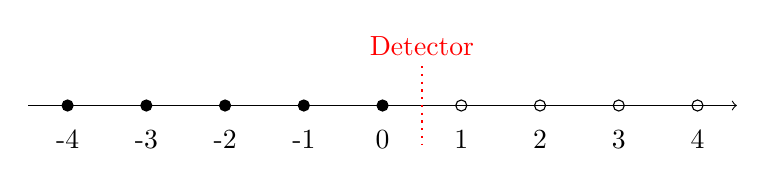
\begin{tikzpicture}[scale=1]
    % Draw the number line
    \draw[->] (-4.5,0) -- (4.5,0);
    \draw[red,thick,dotted](0.5,0.5)node[above]{Detector} -- (0.5,-0.5);
    % Draw filled dots for non-positive integers
    \foreach \x in {-4,...,0} {
        \filldraw[black] (\x,0) circle (2pt);
        \node[below] at (\x,-0.2) {\x};
    }
    
    % Draw hollow dots for positive integers
    \foreach \x in {1,...,4} {
        \draw[black] (\x,0) circle (2pt);
        \node[below] at (\x,-0.2) {\x};
    }
\end{tikzpicture}
    \end{center}

    A strong positive charge at $+\infty$ attracts the electrons independently and identically. Formally, each particle $x_k$ has an internal clock $T_k$ with distribution \[
    \mathbb{P}(T_k> s) = f(s).
    \]
    When the clock rings for $x_k$, $x_k$ will move to the right by one unit, provided that the space in front is empty (not occupied by another electron). The clock then resets to $0$ and $T_k$ is recounted again for the next time the particle moves.
    
    There is a current detector between $0$ and $1$. We want to know the following:
    
    \begin{quote}
        Given time $t>0$, what is the number of particles that passed the current detector? I.e. \[
        y_t \defeq \#\{i:x_i(t)>0\}
        \]
    \end{quote}

\end{aexample}

This was an open question for around 40 years. In the 1940's it was conjectured that \[
y_t \sim ct
\]
for a constant $c$. This was solved in 1988' by Ulm, for the case $\mathbb{P}(T_k\geq s) = e^{-s}$ which is the exponential distribution. In fact, we only understand the cases for $T_k$ is exponentially distributed, or when $T_k$ is geometrically distributed - the former being the limit of the latter. The asymptotics for general $T_k$ is widely open.

\begin{remark}
    I have heard stories about a direct competitor of my firm (one that eats into our profits) giving out this question in an interview with $T_k \sim \text{Geom}(1/2)$. Of course they made it look simple by changing the wording to `decided by a coin flip', like most quant firms. Not sure what they were looking for giving out this question to propsective intern candidates, or maybe I misunderstood and that this question was not even asked - I've never interviewed with them after all.
\end{remark}

\begin{aexample}[breakable=false]{Last Passage Percolation/ LPP}{}
    
\begin{center}
    
    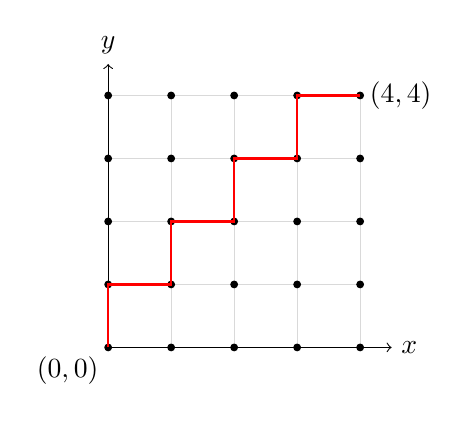
\begin{tikzpicture}[scale=0.8]
    % Draw the grid
    \foreach \x in {0,...,4} {
        \draw[gray!30] (\x,0) -- (\x,4);
    }
    \foreach \y in {0,...,4} {
        \draw[gray!30] (0,\y) -- (4,\y);
    }
    
    % Draw axes with arrows
    \draw[->] (0,0) -- (4.5,0) node[right] {$x$};
    \draw[->] (0,0) -- (0,4.5) node[above] {$y$};
    
    % Draw grid points
    \foreach \x in {0,...,4} {
        \foreach \y in {0,...,4} {
            \filldraw[black] (\x,\y) circle (1.5pt);
        }
    }
    
    % Draw a sample staircase (3,)
    \draw[red, thick] (0,0) -- (0,1) -- (1,1) -- (1,2) -- (2,2) -- (2,3) -- (3,3) -- (3,4)--(4,4);
    
    % Label start and end points
    \node[below left] at (0,0) {$(0,0)$};
    \node[right] at (4,4) {$(4,4)$};
\end{tikzpicture}

\end{center}
\end{aexample}

We now move to a 2-dimensional example. Let us cover all lattice points $v=(x\geq 0,y\geq 0)$ with an IID variable $w_v$. Fix $X,Y$ For each up-right path $\gamma$ from $(0,0) \to (X,Y)$, we let $T(\gamma)\defeq \sum_{v\in \gamma} w_v$.
What are the asymptotics of \[
L(x,y) = \max_{\gamma \text{ from } (0,0)\to (x,y)} T(\gamma)
\]
as $(x,y)\to (\infty,\infty)$, along $x=y$?
\begin{remark}
    You can read \href{https://arxiv.org/pdf/math/9903134}{Johansson} for details on this. (Later, because this spoils the fun)
\end{remark}